\begin{name}
	{\tenchude}
	{TOÁN 12}
	{LỚP TOÁN THẦY PHÁT}
	{Thời gian: 90 phút - Không kể thời gian phát đề}
\end{name}
\Opensolutionfile{ans}[ans/ansDe2-TN1]
\begin{ex}%[2D4N1-1]%[To 20 - Dot 17 - Chuong 4 - Bai 3 - CD - De 1 - TN]%[Nguyễn Hữu Duy]
Cho hàm số $f(x)$ liên tục trên đoạn $[a;c]$ và $b$ là số thực tùy ý thuộc đoạn $[a;c]$. Nếu biết $\displaystyle\int_a^b f(x) \mathrm{\,d}x = 3$ và $\displaystyle\int_b^c f(x) \mathrm{\,d}x = 8$, thì giá trị của $\displaystyle\int_a^c f(x) \mathrm{\,d}x$ là bao nhiêu?
\choice
{\True $11$}
{$-5$}
{$5$}
{$-11$}
\loigiai
{
Ta có $\displaystyle\int_a^c f(x) \mathrm{\,d}x = \displaystyle\int_a^b f(x) \mathrm{\,d}x + \displaystyle\int_b^c f(x) \mathrm{\,d}x = 3 + 8 = 11$.
}
\end{ex}

\begin{ex}%[12-MH-1-MH2025]%[MH-2025, Mã/Tên TV biên soạn]%[2D4N1-2]
Cho hàm số $y = f(x)$ là một nguyên hàm của hàm số $y = x^3$. Phát biểu nào sau đây là đúng?
\choice
{$f(x) = \dfrac{x^4}{4} + C$}
{$f(x) = 3x^2$}
{$f(x) = 4x^3$}
{\True $f(x) = \dfrac{x^4}{4}$}
\loigiai{Hàm số $f(x) = \dfrac{x^4}{4}$ là một nguyên hàm của hàm số $y = x^3$ vì $f'(x) = x^3$.
}
\end{ex}

\begin{ex}%[2D4H1-3]
Tìm nguyên hàm $\displaystyle\int \dfrac{\cos 2x}{\sin^2 x \cos^2 x} \mathrm{d}x$.
\choice
{ $F(x) = -\cos x - \sin x + C$ }
{ $F(x) = \cos x + \sin x + C$ }
{ $F(x) = \cot x - \tan x + C$ }
{\True $F(x) = -\cot x - \tan x + C$ }
\loigiai{
Ta có: $\displaystyle\int \dfrac{\cos 2x}{\sin^2 x \cos^2 x} \mathrm{d}x = \displaystyle\int \left( \dfrac{1}{\sin^2 x} - \dfrac{1}{\cos^2 x} \right) \mathrm{d}x = -\cot x - \tan x + C$.
}
\end{ex}

\begin{ex}%[2D4H2-1]
Tích phân $\displaystyle\int\limits_{1}^{3}\left[2f(x)+1\right]\mathrm{\,d}x=5$ thì $\displaystyle\int\limits_{1}^{3} f(x)\mathrm{\,d}x$ bằng
\choice
{$3$}
{$2$}
{$\dfrac{3}{4}$}
{\True$\dfrac{3}{2}$}
\loigiai{
Ta có
\begin{eqnarray*}
\displaystyle\int\limits_{1}^{3} \left[2f(x)+1\right]\mathrm{\,d}x=5
&\Leftrightarrow&2\displaystyle\int\limits_{1}^{3} f(x)\mathrm{\,d}x+\displaystyle \int_{1}^{3} \mathrm{\,d}x =5\\
&\Leftrightarrow& 2\displaystyle\int\limits_{1}^{3} f(x)\mathrm{\,d}x+\displaystyle 2 =5 \Leftrightarrow \displaystyle\int\limits_{1}^{3} f(x)\mathrm{\,d}x =\dfrac{3}{2}.
\end{eqnarray*}
}
\end{ex}

\begin{ex}%[2D4N3-1]
\immini{Diện tích phần hình phẳng gạch chéo trong hình vẽ bên được tính theo công thức nào?
\choice
{$\displaystyle\int\limits_{-5}^{-3}\left(x+5\right)\mathrm{d}x-\displaystyle\int\limits_{-3}^1\sqrt{1-x}\mathrm{d}x$}
{\True $\displaystyle\int\limits_{-5}^{-3}\left(x+5\right)\mathrm{d}x+\displaystyle\int\limits_{-3}^1\sqrt{1-x}\mathrm{d}x$}
{$\displaystyle\int\limits_{-5}^1\left[\left(x+5\right)-\sqrt{1-x}\right]\mathrm{d}x$}
{$\displaystyle\int\limits_{-5}^1\left[\sqrt{1-x}-\left(x+5\right)\right]\mathrm{d}x$}
}
{
\begin{tikzpicture}[scale=0.8,>=stealth, font=\footnotesize, line join=round, line cap=round]
\def\a{1} \def\b{-3} \def\c{0} \def\d{2} % Hệ số
\def\xmin{-6} \def\xmax{2}
\def\ymin{-1} \def\ymax{5.5}
%	\draw[color=gray!50,dashed] (\xmin,\ymin) grid (\xmax,\ymax);
\draw[->] (\xmin,0)--(\xmax,0) node [below]{$x$};
\draw[->] (0,\ymin)--(0,\ymax) node [left]{$y$};
\node at (0,0) [below left]{$O$};
\clip (\xmin+0.1,\ymin+0.1) rectangle (\xmax-0.5,\ymax-0.1);
\draw[smooth,samples=300,domain=-5.5:1] plot(\x,{sqrt(1-\x)});
\draw[smooth,samples=300] plot(\x,{1*(\x)+5});
\fill[pattern=north east lines,opacity=0.8] (-5,0)--plot[domain=-5:-3](\x,{1*(\x)+5})--plot[domain=-3:1](\x,{sqrt(1-\x)})--(1,0);
\draw[dashed](-3,0)--(-3,2)
;
\draw[fill=black](-3,0)node[below]{$-3$}circle(1pt)
(1,0)node[below]{$1$}circle(1pt)
(-5,0)node[below]{$-5$}circle(1pt)
(-2,3)node[above,rotate=45,scale=0.8]{$y=x+5$}
(-1.5,1.5)node[above,rotate=-20,scale=0.8]{$y=\sqrt{1-x}$}
;
\end{tikzpicture}
}
\loigiai{
Ta chia hình phẳng gạch chéo làm $2$ phần. Nên diện tích hình phẳng là \[ S=\displaystyle\int\limits_{-5}^{-3}\left(x+5\right)\mathrm{d}x+\displaystyle\int\limits_{-3}^1\sqrt{1-x}\mathrm{d}x.\]}
\end{ex}

\begin{ex}%[2D4H3-3]
\immini[thm]{Cho tam giác $OAB$ vuông tại $A$, có cạnh $OA=a$ nằm trên tục $Ox$ và $\widehat{AOB}=\dfrac{\pi}{3}$.
Gọi $\beta$ là khối tròn xoay sinh ra khi quay miền tam giác $OAB$ xung quanh trục $Ox$. Thể tích của khối $\beta$ bằng
\choice
{$3\pi a^3$}
{\True $\pi a^3$}
{$\dfrac{\pi a^3}{3}$}
{$\dfrac{\pi a^3}{9}$}
}{
\begin{tikzpicture}[scale=0.7, font=\footnotesize, line join=round, line cap=round, >=stealth]
\fill[yellow!30]	(0,0)--(4,2)--(4,0)--cycle;
\draw[->] (4,0) -- (5.5,0) node[right] {$x$};
\draw[->] (0,-2.5) -- (0,2.5) node[above] {$y$};
\draw[->] (0,0) -- (-1.5,-1.5) node[below left] {$z$};
\draw (0,0)--(4,2)	(0,0)--(4,-2)	(4,2)--(4,0)	(-0.5,0)--(0,0);
\draw[dashed] (0,0)--(4,0)	;
\draw (4,0) ellipse (0.5 and 2);
\fill (0,0) circle (1pt) node[above left]{$O$};
\fill (4,0) circle (1pt) node[below]{$A$};
\fill (4,2) circle (1pt) node[above]{$B$};
\clip (4,0) -- (0,0) -- (4,2);
\draw (0,0) circle (1cm);
\draw ($(0,0)+(1,0)$) node[above right]{$\alpha$};
%\node[below] at (2.5,-2.5) {Hình $4.31$};
\end{tikzpicture}
}
\loigiai{
Do $OB$ đi qua gốc tọa độ và tạo với $Ox$ một góc $\dfrac{\pi}{3}$ nên $OB\colon y=\tan \dfrac{\pi}{3}x=\sqrt{3} x$.\\
Khi đó, thể tích của khối $\beta$ là
\[
V=\pi \displaystyle\int_0^a\left(\sqrt{3} x\right)^2\mathrm{d}x=\pi \displaystyle\int_0^a3x^2\mathrm{d}x= \pi x^3\bigg|_0^a=\pi a^3.
\]
}
\end{ex}

\begin{ex}%[2H5N1-1]
Trong không gian với hệ toạ độ $Oxyz$, phương trình nào dưới đây là phương trình của mặt phẳng $(Oyz)$?
\choice
{$y=0$}
{\True $x=0$}
{$y-z=0$}
{$z=0$}
\loigiai{
Mặt phẳng $(Oyz)$ đi qua điểm $O(0 ; 0 ; 0)$ và có véc-tơ  pháp tuyến là $\vec{i}=(1 ; 0 ; 0)$ nên ta có phương trình mặt phẳng $(O y z)$ là  $1(x-0)+0(y-0)+0(z-0)=0 \Leftrightarrow x=0$.
}
\end{ex}

\begin{ex}%[2H5N1-2]
Trong không gian $Oxyz$, mặt phẳng nào sau đây nhận véc-tơ $\overrightarrow{n}=(1;2;3)$ làm véc-tơ pháp tuyến?
\choice
{\True $2x+4y+6z=1$}
{$x-2y+3z+1=0$}
{$x+2y-3z-1=0$}
{$2x-4z+6=0$}
\loigiai{
Mặt phẳng $2x+4y+6z=1$ có một véc-tơ pháp tuyến là $\overrightarrow{m}=(2;4;6)$, nên $\overrightarrow{n}=\dfrac{1}{2}\overrightarrow{m}$ cũng là véc-tơ pháp tuyến của mặt phẳng $2x+4y+6z=1$.
}
\end{ex}

\begin{ex}%[2H5H1-3]
Trong không gian với hệ tọa độ $O x y z$, cho điểm $A(2 ; 4 ; 1) ;$ $ B(-1 ; 1 ; 3)$ và mặt phẳng $(P)\colon x-3 y+2 z-5=0$. Một mặt phẳng $(Q)$ đi qua hai điểm $A, B$ và vuông góc với mặt phẳng $(P)$ có dạng $a x+b y+c z-11=0$. Khẳng định nào sau đây là đúng?
\choice
{\True $a+b+c=5$}
{$a+b+c=15$}
{$a+b+c=-5$}
{$a+b+c=-15$}
\loigiai{Vì $(Q)$ vuông góc với $(P)$ nên $(Q)$ nhận véc-tơ pháp tuyến $\vec{n}=(1 ;-3 ; 2)$ của $(P)$ làm véc-tơ chỉ phương.\\
Mặt khác $(Q)$ đi qua $A$ và $B$ nên $(Q)$ nhận $\overrightarrow{A B}=(-3 ;-3 ; 2)$ làm véc-tơ chỉ phương.\\
$(Q)$ nhận $\overrightarrow{n}_Q=[\vec{n}, \overrightarrow{A B}]=(0 ; 8 ; 12)$ làm véc-tơ pháp tuyến.\\
Vậy phương trình mặt phẳng $(Q)\colon  0(x+1)+8(y-1)+12(z-3)=0\Leftrightarrow 2 y+3 z-11=0$.\\
Vậy $a+b+c=5$.}
\end{ex}

\begin{ex}%[2H5N2-1]%[Dự án 2025 - Đề cấu trúc mới của Bộ theo [Thành Đức Trung]
Trong không gian $Oxyz$, đường thẳng $d\colon \heva{ & x=1+2t \\ & y=3-t \\ & z=1-t}$ $(t\in \mathbb{R})$ đi qua điểm nào dưới đây?
\choice
{$M(1;3;-1)$}
{\True $N(-3;5;3)$}
{$P(3;5;3)$}
{$Q(1;2;-3)$}
\loigiai
{
Thay tọa độ các điểm vào phương trình $d$, ta có $\heva{ & -3=1+2t \\ &5=3-t \\ & 3=1-t} \Leftrightarrow t=-2$. \\
Vậy $N(-3;5;3)\in d$.
}
\end{ex}

\begin{ex}%[2H5N2-7]
Trong không gian với hệ trục $Oxyz$, cho hai đường thẳng $d_1:\dfrac{x}{1}=\dfrac{y+1}{-1}=\dfrac{z-1}{2}$ và $d_2:\dfrac{x+1}{-1}=\dfrac{y}{1}=\dfrac{z-3}{1}$. Góc giữa hai đường thẳng đó bằng
\choice
{$45^\circ $}
{\True $90^\circ $}
{$60^\circ $}
{$30^\circ $}
\loigiai{
Đường thẳng $d_1$ có véctơ chỉ phương $\overrightarrow{u}_1=\left( 1;-1;2 \right)$.\\
Đường thẳng $d_2$ có véctơ chỉ phương $\overrightarrow{u}_2=\left( -1;1;1 \right)$.\\
Gọi $\alpha$ là góc giữa hai đường thẳng trên.\\
Khi đó ta có $\cos \alpha =\left| \cos \left( \overrightarrow{u}_1,\overrightarrow{u}_2 \right) \right|=\dfrac{\left| 1\cdot\left( -1 \right)+\left( -1 \right)\cdot1+2\cdot1 \right|}{\sqrt{1^2+{{\left( -1 \right)}^2}+2^2}\cdot\sqrt{{{\left( -1 \right)}^2}+1^2+1^2}}=0$.\\$\Rightarrow \left( \widehat{d_1,d_2} \right)=90^\circ $.}
\end{ex}

\begin{ex}%[2H5H2-4]
Trong không gian $Oxyz$ cho đường thẳng $\Delta  \colon \dfrac{x}{1} =\dfrac{y+1}{2} =\dfrac{z-1}{1} $ và mặt phẳng $\left(P\right) \colon x-2y-z+3=0$. Đường thẳng nằm trong $\left(P\right)$ đồng thời cắt và vuông góc với $\Delta $ có phương trình là
\choice
{$\heva{x&=1+2t \\ y&=1-t \\ z&=2} $}
{$\heva{x&=-3 \\ y&=-t \\ z&=2t} $}
{$\heva{x&=1+t \\ y&=1-2t \\ z&=2+3t} $}
{\True $\heva{x&=1 \\ y&=1-t \\ z&=2+2t} $}
\loigiai{
Ta có $\Delta  \colon \dfrac{x}{1} =\dfrac{y+1}{2} =\dfrac{z-1}{1} $$\Rightarrow \Delta  \colon \heva{x&=t \\ y&=-1+2t \\ z&=1+t.} $ \\
Gọi $M=\Delta \cap \left(P\right)$ $\Rightarrow M\in \Delta \Rightarrow M\left(t;2t-1;t+1\right)$ $M\in \left(P\right)\Rightarrow t-2\left(2t-1\right)-\left(t+1\right)+3=0 \Leftrightarrow 4-4t=0\Leftrightarrow t=1\Rightarrow M\left(1;1;2\right)$. \\
Véc-tơ pháp tuyến của mặt phẳng $\left(P\right)$ là $\overrightarrow{n}=\left(1;-2;-1\right)$. \\
Véc-tơ chỉ phương của đường thẳng $\Delta $ là $\overrightarrow{u}=\left(1;2;1\right)$.\\
Đường thẳng $d$ nằm trong mặt phẳng $\left(P\right)$ đồng thời cắt và vuông góc với $\Delta $. \\
$\Rightarrow $ đường thẳng $d$ nhận $\dfrac{1}{2} \left[\overrightarrow{n},\overrightarrow{u}\right]=\left(0;-1;2\right)$ làm véc-tơ chỉ phương và $M\left(1;1;2\right)\in d$.\\
$\Rightarrow $ Phương trình đường thẳng $d \colon \heva{x&=1 \\ y&=1-t \\ z&=2+2t.}$}
\end{ex}
\Closesolutionfile{ans}

\TNTF
\Opensolutionfile{ans}[ans/ansDe2-TN2]
\begin{ex}%[2D4H2-4]%[Tổ 20 - Đợt 17 - Chương 4 - - CD - Đề 6]%[Nắng Đông]
Cho $A=\displaystyle\int\limits_0^1 \dfrac{3}{2^x} \mathrm{\,d}x$ và  $B=\displaystyle\int\limits_0^1 4\mathrm{e}^{-2x} \mathrm{\,d}x$.
\choiceTF[t]
{\True $A=-\dfrac{3}{2^x\ln 2}\bigg|_0^1$}
{$B=\dfrac{2}{\mathrm{e}^{2x}}\bigg|_0^1$}
{$A=-\dfrac{3}{2\ln 2}$}
{\True $B=a+\dfrac{b}{\mathrm{e}^2}$, với $a$, $b$ là các số nguyên thì $a\cdot b = -4$}
\loigiai
{Ta có $A=\displaystyle\int\limits_0^1 \dfrac{3}{2^x} \mathrm{\,d}x
= \displaystyle\int\limits_0^1 {3\cdot \left(\dfrac{1}{2}\right)^x} \mathrm{\,d}x
= \dfrac{3}{2^x\ln \dfrac{1}{2}}\bigg|_0^1
=-\dfrac{3}{2^x\ln 2}\bigg|_0^1
= \dfrac{3}{2\ln 2}$.\\
Và $B=\displaystyle\int\limits_0^1 4\mathrm{e}^{-2x} \mathrm{\,d}x
=\displaystyle\int\limits_0^1 4\left(\mathrm{e}^{-2}\right)^x \mathrm{\,d}x
= 4\cdot \dfrac{\left(\mathrm{e}^{-2}\right)^x}{\ln \mathrm{e}^{-2}}\bigg|_0^1
= -\dfrac{2}{\mathrm{e}^{2x}}\bigg|_0^1
=2 - \dfrac{2}{\mathrm{e}^2}$.
\begin{itemchoice}
\itemch Đúng.
\itemch Sai.
\itemch Sai.
\itemch Đúng. Vì $a=2$, $b=-2$ suy ra $a\cdot b = -4$.
\end{itemchoice}
}
\end{ex}

\begin{ex}%[Dat Thai, Dự án Ex-TF-TLN-2024-Dot03]%[2H5H2-5]
Cho đường thẳng $d\colon \heva{& x = 1 + t\\& y = 2 - t\\& z = 1 + 2t}, t\in \mathbb{R}$ và mặt phẳng $(P)\colon x + 2y + z - 5 = 0$. Tọa độ giao điểm $A$ của đường thẳng $d$ và mặt phẳng $(P)$ là $(a;b;c)$.
\choiceTF
{\True $a+b+c = 2$}
{\True Có đúng $1$ số dương trong ba số $a$, $b$, $c$}
{$a$ là số lớn nhất trong ba số $a$, $b$, $c$}
{$a$, $b$, $c$ theo thứ tựu lập thành một cấp số cộng}
\loigiai{
Tọa độ giao điểm $A$ của đường thẳng $d$ và mặt phẳng $P$ là nghiệm của hệ phương trình sau
\begin{eqnarray*}
\heva{& x = 1 + t\\& y = 2 - t\\ & z = 1 + 2t \\& z + 2y + z -5 = 0} \Leftrightarrow \heva{& t  =-1\\& x = 0\\& y = 3 \\& z = -1} \Rightarrow A(0; 3; -1).
\end{eqnarray*}
Vậy
\begin{itemchoice}
\itemch \textbf{Đúng}.
\itemch \textbf{Đúng}. Vì chỉ có mỗi $b$ là số dương trong ba số $a$, $b$, $c$.
\itemch \textbf{Sai}. Vì $b$ là số lớn nhất trong ba số $a$, $b$, $c$.
\itemch \textbf{Sai}. Vì $2b \ne a+ c$.
\end{itemchoice}
}
\end{ex}
\Closesolutionfile{ans}

\TNSA
\Opensolutionfile{ans}[ans/ansDe2-TN3]
\begin{ex}%[2D4H1-1]%[Đào Trung Kiên]
Biết $F(x)$ là một nguyên hàm của hàm số $f(x)=\sin x$ và đồ thị hàm số $y=F(x)$ đi qua điểm $M\left(0;1\right)$. Tính $F\left(\dfrac{\pi}{2}\right)$ (làm tròn kết quả tới hàng đơn vị).
\shortans[]{$2$}
\loigiai{
Ta có $F(x)=\displaystyle\int f(x)\mathrm{\,d}x=-\cos x+C$.\\
Mà đồ thị hàm số $y=F(x)$ đi qua $M(0;1)$ nên $F(0)=1\Leftrightarrow -1+C=1\Leftrightarrow C=2$.\\
Suy ra $F(x)=-\cos x+2$ nên $F\left(\dfrac{\pi}{2}\right)=2$.}
\end{ex}

\begin{ex}%[2D4V3-2]
\immini{
Sàn của một viện bảo tàng mỹ thuật được lát bằng những viên gạch hình vuông cạnh $40$ cm  như hình bên. Biết rằng người thiết kế đã sử dụng các đường cong có phương trình $4x^2=y^4$  và  $4y^2 =x^4$ để tạo hoa văn cho viên gạch. Tính diện tích (đơn vị cm$^2$) phần được tô đậm (làm tròn kết quả đến hàng đơn vị).
}
{
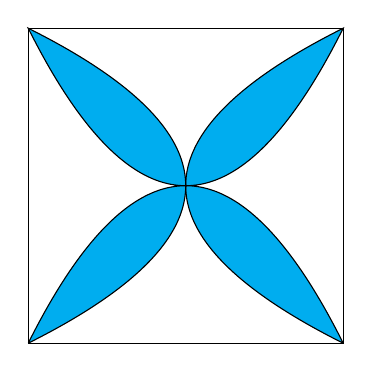
\begin{tikzpicture}
\draw (2,2)--(2,-2)--(-2,-2)--(-2,2)--cycle;
\draw[fill=cyan, smooth, samples=200] plot[domain=-2:2,variable=\y]({0.5*(\y)^2},{\y})--plot[domain=2:0,variable=\x]({\x},{0.5*(\x)*(\x)})--plot[domain=0:2,variable=\x]({\x},{(-0.5)*(\x)*(\x)});
\draw[fill=cyan, smooth, samples=200] plot[domain=-2:2,variable=\y]({-0.5*(\y)^2},{\y})--plot[domain=-2:0,variable=\x]({\x},{0.5*(\x)*(\x)})--plot[domain=0:-2,variable=\x]({\x},{(-0.5)*(\x)*(\x)});
\end{tikzpicture}
}
\shortans{$533$}
\loigiai{
\immini{
Do tính đối xứng nên diện tích cần tìm bằng $4$ lần diện tích phần tô đậm của hình vẽ bên. Ta chỉ xét đồ thị trong góc phần tư thứ nhất do đó
\begin{align*}
&4x^2=y^4 \Leftrightarrow y = \sqrt{2x} \\
&4y^2 =x^4 \Leftrightarrow  y = \dfrac{1}{2} x^2.
\end{align*}
}
{
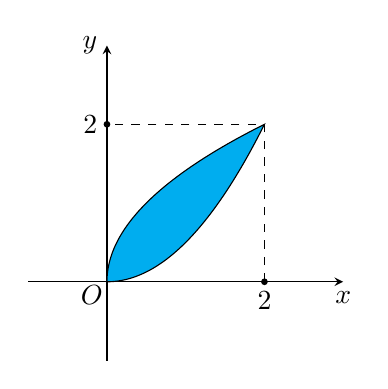
\begin{tikzpicture}[scale=1,>=stealth]
\draw[->] (-1,0)--(3,0) node[below] {$x$};
\draw[->] (0,-1)--(0,3) node[left] {$y$};
%\draw[fill] (1,0) circle (1pt) node[below] {$1$};
\draw[fill] (0,0) circle node[below left=-2pt] {$O$};
\draw[dashed] (2,0)--(2,2)--(0,2);
\draw[fill] (2,0) circle (1pt) node[below] {$2$};
\draw[fill] (0,2) circle (1pt) node[left] {$2$};
\draw[fill=cyan, smooth, samples=200] plot[domain=0:2,variable=\y]({0.5*(\y)^2},{\y})--plot[domain=2:0,variable=\x]({\x},{0.5*(\x)*(\x)});
\end{tikzpicture}
}
\noindent Một đơn vị trong hệ tọa độ $Oxy$ bằng $10$ cm, do đó diện tích của phần tô đậm ban đầu là
\[
S =4\cdot 10^2 \int \limits_0^2 \left ( \sqrt{2x}-\dfrac{1}{2}x ^2\right) \mathrm{d}x = 400 \left ( \dfrac{2\sqrt{2}}{3} \sqrt{x^3}-\dfrac{1}{6}x^3 \right ) \Bigg|_0^2= \dfrac{1600}{3}\approx 533 \ \mathrm{(cm^2)}.
\]
}
\end{ex}

\begin{ex}%[2H5H2-7]
Số các mặt phẳng $(\alpha)$ chứa đường thẳng $d\colon\dfrac{x}{1}=\dfrac{y}{-1}=\dfrac{z}{-3}$ và tạo với mặt phẳng $(P)\colon 2x-z+1=0$ góc $45^\circ $ bằng
\shortans{$2$}
\loigiai{
Đường thẳng $d$ đi qua điểm $O(0;0;0)$ có véc-tơ chỉ phương $\overrightarrow{u}=(1;-1;-3)$.\\
Ta có $(\alpha)$ qua $O$ có véc-tơ pháp tuyến $\overrightarrow{n}=(a;b;c)$ có dạng $ax+by+cz=0$.\\
Vì $\overrightarrow{n}\perp \overrightarrow{u}$ nên $\overrightarrow{n}\cdot \overrightarrow{u}=0$. Do đó $ a-b-3c=0$.\\
Mặt phẳng $(P)\colon 2x-z+1=0$ có véc-tơ pháp tuyến $\overrightarrow{k}=(2;0;-1)$.\\
Ta có
\begin{eqnarray*}
&&\cos 45^\circ =\dfrac{\left| \overrightarrow{n}\cdot \overrightarrow{k}\right|}{\left|\overrightarrow{n}\right|\cdot\left|\overrightarrow{k}\right|}\\
&\Leftrightarrow&\dfrac{\left| 2a-c\right|}{\sqrt{5(a^2+b^2+c^2)}}=\dfrac{\sqrt{2}}{2}\\
&\Leftrightarrow&10(a^2+b^2+c^2)=(4a-2c)^2\\
&\Leftrightarrow&10(b^2+6bc+9c^2+b^2+c^2)=(4b+12c-2c)^2\\
&\Leftrightarrow&10(2b^2+6bc+10c^2)=(4b+10c)^2\\
&\Leftrightarrow&4b^2-20bc=0\\
&\Leftrightarrow&\hoac{&b=0 \\&b=5c.}
\end{eqnarray*}
Xét
\begin{itemize}
\item $b=0\Rightarrow a=3c$ nên $(\alpha)\colon x+3z=0$.
\item $b=5c$, chọn $c=1\Rightarrow b=5$, $a=8$ nên $(\alpha)\colon 8x+5y+z=0$.
\end{itemize}
}
\end{ex}

\begin{ex}%[12-MH-2-MH2025]%[MH-2025, Nguyễn Trần Phong]%[2H5V1-7]
Một phần sân nhà bác An có dạng hình thang $ABCD$ vuông tại $A$ và $B$ với độ dài $AB=9$ m, $AD=5$ m và $BC=6$ m. Theo thiết kế ban đầu thì mặt sân bằng phẳng và $A$, $B$, $C$, $D$ có độ cao như nhau. Sau đó bác An thay đổi thiết kế để nước có thể thoát về phía góc sân ở vị trí $C$ bằng cách giữ nguyên độ cao ở $A$, giảm độ cao của sân ở vị trí $B$ và $D$ xuống thấp hơn độ cao ở $A$ lần lượt là $6$ cm và $3{,}6$ cm. Để mặt sân sau khi lát gạch vẫn là bề mặt phẳng thì bác An cần phải giảm độ cao ở $C$ xuống bao nhiêu cen-ti-mét so với độ cao ở $A$? \textit{Kết quả làm tròn đến hàng phần mười)}
\shortans{$10{,}3$}
\indent\indent\indent\indent\indent\indent\indent\indent\indent\begin{tikzpicture}[scale=0.5, font=\footnotesize,line join=round, line cap=round, >=stealth]
\path
(0,0) coordinate (A)
(9,0) coordinate(B)
(9,-6) coordinate(C)
(0,-5) coordinate(D)
;
\draw[thick] (A)--(B)--(C)--(D)--cycle;
\node [above] at ($(A)!0.5!(B)$) {$9$ m};
\node [right] at ($(B)!0.5!(C)$) {$6$ m};
\node [left] at ($(A)!0.5!(D)$) {$5$ m};
\foreach \i/\g in {A/90,B/90,C/-90,D/-90}{\draw[fill=black](\i) circle (0pt) ($(\i)+(\g:4mm)$) node[scale=1]{$\i$};}
\end{tikzpicture}
\loigiai{
Tại vị trí ban đầu $A$, $B$, $C$, $D$ có độ cao như nhau, chọn hệ trục tọa độ có gốc tọa độ là điểm $A$ và các trục tọa độ lần lượt là $AD$, $AB$ và $Az$, với $Az \perp (ABCD)$.\\
Khi đó $A(0 ; 0 ; 0)$, $D(5; 0 ; 0)$, $B(0; 9 ; 0)$, $C(6; 9 ; 0)$.\\
Sau đó bác An thay đổi thiết kế để nước có thể thoát về phía góc sân ở vị trí $C$ bằng cách giữ nguyên độ cao ở $A$, giảm độ cao của sân ở vị trí $B$ và $D$ xuống thấp hơn độ cao ở $A$ lần lượt là $6$ cm và $3{,}6$ cm.\\
Khi đó, $A(0 ; 0 ; 0)$, $D(5; 0 ; -3{,}6)$, $B(0; 9 ; -6)$.\\
Ta có $\overrightarrow{AB}=(0 ; 9 ; -6)$, $ \overrightarrow{AD}=(5 ; 0 ; -3{,}6)$ là cặp véc-tơ chỉ phương của mặt phẳng $(ABD)$ nên một véc-tơ pháp tuyến của $(ABD)$ là $\left[\overrightarrow{AB}, \overrightarrow{AD}\right]=(-32{,}4 ; -30 ; -45)$.\\
Vậy mặt phẳng $(ABD)$ qua $A(0 ; 0 ; 0)$ và có véc-tơ pháp tuyến $\vec{n}=(-32{,}4 ; -30 ; -45)$ nên có phương trình là
\allowdisplaybreaks
\begin{eqnarray*}
-32{,}4 (x-2)-30(y+1)-45(z-3)=0 \qquad \text{hay } -32{,}4 x -30y -45z=0.
\end{eqnarray*}
Để mặt sân sau khi lát gạch vẫn là bề mặt phẳng thì bác An cần phải giảm độ cao ở $C$ xuống $k$ centimét so với độ cao ở $A$ nên suy ra $C(6; 9 ; -k)$.\\
Ta có $A$, $B$, $C$, $D$ đồng phẳng\\
$\Leftrightarrow C \in (ABD)$\\
$\Leftrightarrow -32{,}4\cdot 6 -30 \cdot 9 -45\cdot (-k)=0$\\
$\Leftrightarrow k=10{,}32$.\\
Vậy bác An cần phải giảm độ cao ở $C$ xuống $10{,}3$ cen-ti-mét so với độ cao ở $A$.
}\end{ex}

\TL
\begin{ex} %[2H5H2-3].
Trong không gian $Oxyz$, cho ba điểm $A(3 ;-2 ;-2), B(3 ; 2 ; 0), C(0 ; 2 ; 1)$. Phương trình mặt phẳng $(ABC)$ có dạng $=ax+by+cz+d=0$. Tính $a+b+c$.
\shortans{$5$}
\loigiai{
Ta có $\overrightarrow{AB}=(0 ; 4 ; 2), \overrightarrow{AC}=(-3 ; 4 ; 3), \overrightarrow{n}=\left[ \overrightarrow{B} ; \overrightarrow{C}\right]=(4 ;-6 ; 12)$.\\
Ta có $\overrightarrow{n}=(4 ;-6 ; 12)$ cùng phương $\overrightarrow{n}_{1}=(2 ;-3 ; 6)$.\\
Mặt phẳng $(ABC)$ đi qua điểm $C(0 ; 2 ; 1)$ và có một véc-tơ pháp tuyến $\overrightarrow{n}_{1}=(2 ;-3 ; 6)$ nên $(ABC)$ có phương trình là
\[2(x-0)-3(y-2)+6(z-1)=0 \Leftrightarrow 2 x-3 y+6 z=0.\]
Vậy phương trình mặt phẳng cần tìm là $2x-3y+6z=0$.\\
Suy ra $a+b+c=5$.
}
\end{ex}

\begin{ex}%[2D4C3-2]
	\immini[thm]{Một họa tiết hình cánh bướm như hình vẽ bên. Phần tô đậm được đính đá với giá thành $500\,000$/$\,\mathrm{m^2}$. Phần còn lại được tô màu với giá thành $250\,000$/$\,\mathrm{m^2}$. Cho $AB=4$\,dm; $BC=8$\,dm. Hỏi để trang trí $1\,000$ họa tiết như vậy cần số tiền là bào nhiêu? (làm tròn đến hàng nghìn)
	% \choice
	% {$105\,660\,667$}
	% {\True $106\,666\,667$}
	% {$ 107\,665\,667$}
	% {$ 108\,665\,667$}
	}{
	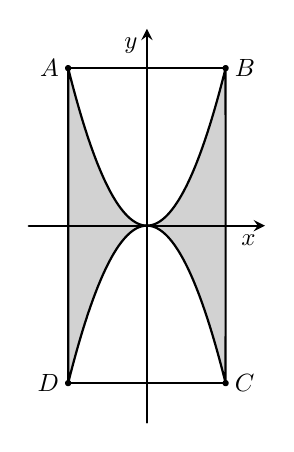
\begin{tikzpicture}[line join=round, line cap=round,>=stealth,thick,scale=0.5]
	\tikzset{every node/.style={scale=0.9}}
	\begin{scope}
	\draw[fill=gray!35](-2,0)--plot[samples=200,domain=-2:2,smooth,variable=\x] (\x,{(\x)^2})--(2,0);
	\draw[fill=gray!35](-2,0)--plot[samples=200,domain=-2:2,smooth,variable=\x] (\x,{-1*(\x)^2})--(2,0);
	\draw[fill=black](-2,4) circle (1.5pt) node[left]{$A$} (2,4) circle (1.5pt) node[right]{$B$} (2,-4) circle (1.5pt) node[right]{$C$} (-2,-4) circle (1.5pt) node[left]{$D$};
	\draw (-2,4)--(2,4) (2,-4)--(-2,-4);
	\end{scope}
	\draw[->] (-3,0)--(3,0) node[below left] {$x$};
	\draw[->] (0,-5)--(0,5) node[below left] {$y$};
	\end{tikzpicture}
	}
	\loigiai{
	Vì $AB=4$\,dm; $BC=8$\,dm $\Rightarrow A(-2;4)$, $B(2;4)$, $C(2;-4)$, $D(-2;-4)$.\\
	parabol là $y=x^2$ hoặc $y=-x^2$.\\
	Diện tích phần tô đậm là $S_1=4\displaystyle\int\limits_0^2{x^2}\mathrm{\,d}x=\dfrac{32}{3}\mathrm{\,(dm^2)}$.\\
	Diện tích hình chữ nhật là $S=4\cdot 8=32\mathrm{\,(dm^2)}$.\\
	Diện tích phần trắng là $S_2=S-S_1=32-\dfrac{32}{3}=\dfrac{64}{3}\mathrm{\,(dm^2)}$.\\
	Tổng chi phí trang chí là $T=\left(\dfrac{32}{3}\cdot 5\,000+\dfrac{64}{3}\cdot 2\,500\right)\cdot 1\,000\approx 106\,667\,000$.
	}
	\end{ex}

\begin{ex}%[Mức độ ]giảng 12 New - 4in1, Đoàn Hùng]%[2H5V1-7]
	\immini
	{Trong không gian với hệ tọa độ $Oxyz$ (đơn vị trên mỗi trục toạ độ là km), một máy bay đang ở vị trí $A(3;-2{,}5; 0{,}5)$ và sẽ hạ cánh ở vị trí $B(3; 7{,}5; 0)$ trên đường băng (hình bên). Có một lớp mây được mô phỏng bởi một mặt phẳng $(\alpha)$ đi qua ba điểm $M(9;0;0)$, $N(0;-9;0)$, $P(0;0;0{,}9)$. Tính độ cao của máy bay khi máy bay xuyên qua đám mây để hạ cánh.}
	{\begin{tikzpicture}[line join = round, line cap = round,>=stealth,font=\footnotesize,scale=.5]
	\path
	(0,0) coordinate (O)
	(-9,0) coordinate (N)
	($(O)!1!40:(N)$) coordinate (M)
	(0,0.9) coordinate (P)
	($(O)!1.2!(M)$) coordinate (x)
	(-5,0.8) coordinate (A)
	(4,-1.5) coordinate (B)
	($(A)!2.1cm!(B)$) coordinate (C)
	(intersection of A--B and O--M) coordinate (B1)
	;
	\draw[line width=0.3mm,red] (A)--(C) (B1)--(B);
	\draw[line width=0.3mm,red,dashed] (C)--(B1);
	\draw[->,>=stealth,line width=0.3mm,blue] (0,0)--(x) node[right=0.2cm]{$x$};
	\draw[->,>=stealth,line width=0.3mm,blue] (-10,0)--(-9,0) (0,0) node[above right]{$O$}--(7,0) node[below]{$y$};
	\draw[line width=0.3mm,blue,dashed] (-9,0)--(0,0);
	\draw[->,>=stealth,line width=0.3mm,blue] (0,0)--(0,3) node[left]{$z$};
	\draw[line width=0.3mm,blue] (N)--(P)--(M) (N)--(M);
	\foreach \x/\gm in {N/90,P/140} \fill (\x) circle (1pt) ($(\x)+(\gm:5mm)$)node[blue]{$\x$};
	\filldraw[red] (N)node[below left,blue]{$-9$} (P)node[blue,above right]{$0{,}9$} (M)node[blue,right=0.1cm]{$9$}node[blue,left=0.1cm]{$M$} (C) circle (3pt) node[below=0.2cm,blue]{\scriptsize $C$} (A) circle (3pt)node[above left,red,blue]{$A$} (B)circle (3pt) node[below,blue]{$B$};
	\end{tikzpicture}}
	% \shortans{$0{,}45$}
	\loigiai{
	Giả sử điểm $C\left(x_C;y_C;z_C\right)$ là vị trí mà máy bay xuyên qua đám mây để hạ cánh, suy ra $C\in (\alpha)$. Áp dụng phương trình mặt phẳng theo đoạn chắn, ta thấy mặt phẳng $(\alpha)$ có phương trình là
	\[\dfrac{x}{9}-\dfrac{y}{9}+\dfrac{z}{0{,}9}=1 \Leftrightarrow x-y+10z=9 \Rightarrow x_C-y_C+10z_C=9.\]
	Mặt khác, vì $\vec{AC}$, $\vec{AB}$ là hai véc-tơ cùng hướng nên tồn tại số thực $t>0$ sao cho $\vec{AC}=t\cdot \vec{AB}$.\\
	Do $\vv{AC}=\left(x_C-3;y_C+2{,}5;z_C-0{,}5\right)$; $\vv{AB}=\left(3-3;7{,}5+2{,}5;0-0{,}5\right)=\left(0;10;-0{,}5\right)$\\
	nên $\heva{&x_C-3=0t\\&y_C+2{,}5=10t\\&z_C-0{,}5=-0{,}5t} \Leftrightarrow \heva{&x_C=3\\&y_C=10t-2{,}5\\&z_C=-0{,}5t+0{,}5.}$\\
	Vì $C\in(\alpha)$ nên $3-(10 t-2{,}5)+10(-0{,}5 t+0{,}5)=9 \Leftrightarrow t=0{,}1$. Suy ra $C(3;-1{,}5;0{,}45)$.\\
	Vậy tại vị trí $C$, độ cao của máy bay là $0{,}45$ km.
	}
	\end{ex}
\Closesolutionfile{ans}


% \Closesolutionfile{ansbook}
% \HetDe
% \label{De2}
% %
% \cleardoublepage
% \setcounter{page}{1}
% \rfoot{Trang \thepage/\pageref{DA2} - Đáp án trắc nghiệm Mã đề 2}
% \begin{center}
% 	\bfseries ĐÁP ÁN TRẮC NGHIỆM MÃ ĐỀ 2
% \end{center}

% \inputansbox{10}{ans/ansDe2-TN1}
% \inputansbox[3]{2}{ans/ansDe2-TN2}
% \inputansbox{3}{ans/ansDe2-TN3}
% \label{DA2}
% %
